\newpage
\section{Dynamic Routing}
\subsection{Dynamic Routing의 개념}
    관리자가 직접 경로를 입력할 필요 없이 Router들이 Dynamic Routing Protocol에 따라 자동으로 서로의 네트워크 정보를 교환하여 네트워크 정보를 업데이트하고 최적의 경로를 결정하는 Routing 방식이다. \\
    Dynamic Routing Protocol은 AS 내에서 사용하는 IGP와 AS 사이에서 사용하는 EGP로 나눌 수 있고, IGP Routing Protocol은 동작 방식에 따라 Distance Vector와 Link State 방식이 있다. Distance vector 방식은 거리와 방향 정보를 기준으로 최적 경로를 탐색하며, 대표적인 프로토콜로 RIP, IGRP, BGP가 있다. Link State 방식은 연결 상태 (대역폭) 정보로 최적 경로를 탐색하며, 대표적인 프로토콜로 OSPF, IS-IS가 있다. \\
    각 Routing Protocol들은 최적의 경로를 선택하는 기준이 다르기 때문에 서로 다른 Routing Protocol은 서로 정보를 교환하지 않는다. \\
    
    \vspace{-4mm}
    \begin{figure}[!h]\centering
		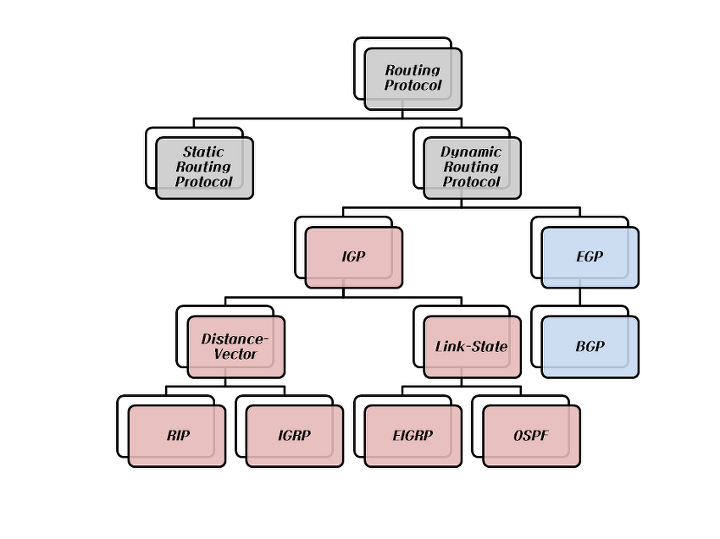
\includegraphics[width=.65\textwidth]{image/week06/4-1.png}
		\caption{\small Routing Protocol}
		\vspace{-10pt}
    \end{figure}
    
\subsection{Dynamic Routing의 장단점}
    \subsubsection*{장점}
    라우팅 경로 계산을 위한 장비나 리소스를 요구하지 않는다. \\
    Routing  Table 교환할 필요가 없어 대역폭을 절약할 수 있고 보안에 좋다. \\
    \subsubsection*{단점}
    경로가 단절된 경우 관리자가 직접 대안의 경로를 입력해야한다. \\
    대규모 네트워크/다중 경로 구성/유동적인 네트워크 구성에 부적합하다. \\
\newpage